\begin{landscape}
    \chapter{Quantum Physics}
    \begin{itemize}
        \item[\AsteriskThin] \emph{A photon} is defined as \emph{a quantum} of electromagnetic energy. A photon of frequency \(f\) has energy \(E=hf\), where \(h\) is Planck's constant. 
        \item Planck's constant \(h=6.63\cdot 10^{-34}\) Js. A useful conversion: 1 eV\({}=1.60\cdot 10^{-19}\) J 
        \item[\AsteriskThin] \emph{The photoelectric effect} refers to the emission of \emph{electrons from a metal surface} when the surface is \emph{irradiated} with electromagnetic radiation of a \emph{high enough frequency}.
    \end{itemize}
    \begin{longtable}{
        |m{21.7624088777cm*\real{0.25}}|m{21.7624088777cm*\real{0.32}};{2pt/2pt}M{21.7624088777cm*\real{0.03}}|m{21.7624088777cm*\real{0.4}}|
        % |M{21.7624088777cm*\real{0.3}}|M{21.7624088777cm*\real{0.7}}|
        }
        \hline
        \begin{minipage}{21.7624088777cm*\real{0.25}}
            \centering
            Experimental observations
        \end{minipage}& 
        \multicolumn{2}{Sc|}{Predictions of classical theory}&
        \begin{minipage}{21.7624088777cm*\real{0.4}}
            \centering
            Explanation via quantum theory
        \end{minipage}\\ 
        % Experimental observations & Explanation via quantum theory\\ 
        \hline
        \begin{itemize}
            \item \emph{Emission} of photoelectrons is almost \emph{instantaneous}, with a negligible time lag.
            \item Is unaffected by the intensity or brightness of the light if the light is above the threshold frequency.
        \end{itemize}&
        \begin{itemize}
            \item Electrons should absorb energy over a period of time before it gains enough energy to escape the metal.
            \item A dim light after some delay would transfer sufficient energy to the electron for ejection, whereas a very bright light would eject electrons after a short while.
        \end{itemize}&
        \textcolor{red}{\(\times\)}&
        \begin{itemize}
            \item Photon-electron interaction is \emph{one-to-one}.
            \item Energy of a single photon cannot be shared; it either gives up all of its energy to the electron, or none at all.
            \item This absorption of the photon then leads to a gain in energy for the electron.
            \item The time taken for the electron to gain sufficient energy is negligible. Hence, photoemission is \emph{instantaneous}.
        \end{itemize}\\
        \hline
        \begin{itemize}
            \item Electrons are emitted when the frequency of light is above the \emph{threshold frequency} \(f_0\) (or below the threshold wavelength \(\lambda_0\)).
            \item No electron is emitted below \(f_0\), \emph{regardless of the light intensity}.
        \end{itemize}&
        \begin{itemize}
            \item Energy of the wave is dependent on the square of its amplitude. 
            \item Electrons \emph{will} absorb enough energy to escape given \emph{sufficient time}.
            \item There should \emph{not} be any threshold frequency. 
        \end{itemize}&
        \textcolor{red}{\(\times\)}&
        \begin{itemize}
            \item The existence of the threshold frequency again traces back to the \emph{one-to-one} interactions between electrons and photons. 
            \item[\AsteriskThin] \emph{The work function} \(\phi\) is the \emph{minimum energy} required to eject/free an electron from the \emph{surface} of a metal.
            \item \emph{Note.} The energy \(E\geq\phi\) required to free an electron \emph{varies} from electron to electron.
        \end{itemize}\\
        \hline
        The \emph{maximum kinetic energy} of the ejected electrons is independent of the \emph{intensity} of the light, but dependent on the \emph{frequency} of the light.&
        The higher the light \emph{intensity}, the higher the \emph{energy} of the light wave striking the metal surface. Electrons should be ejected with \emph{greater} kinetic energy. It \emph{cannot} explain why the maximum kinetic energy is dependent on frequency and independent of intensity.&
        \textcolor{red}{\(\times\)}&
        \begin{itemize}
            \item By the conservation of energy, energy imparted by a photon is used to \emph{free} the electron and becomes the \emph{kinetic energy} of the emitted electron.
            \item For an electron requiring the \emph{minimum} energy \(\phi\) to escape from the metal, its kinetic energy will be a \emph{maximum}. i.e. \(hf=\phi+E_{k,\text{max}}\).
            \item When the light source increases in \emph{frequency}, the \emph{energy} \(E_{\text{photon}}\propto f\) of the emitted \emph{photons} increases proportionately. So, the \emph{maximum} kinetic energy \(E_{k,\text{max}}=E_{\text{photon}}-\phi\) of the electrons emitted also increases. 
        \end{itemize}\\
        \hline
        The \emph{rate} at which electrons were ejected, and therefore, the \emph{photocurrent} produced is proportional to the \emph{intensity} of the light.&
        A higher light intensity should be able to simultaneously free more electrons from the metal at any instant. This results in a higher current.&
        \textcolor{green!70!black}{\checkmark}&
        The \emph{intensity} of the \emph{monochromatic} light beam is directly proportional to the number of \emph{photons} passing through a cross-sectional \emph{area} per unit \emph{time}. In fact,
        \[I=\frac{N}{t}\cdot\frac{hf}{A}=\frac{Nhf}{tA}.\]
        The higher the light \emph{intensity}, the higher the \emph{number of photons per unit time} hitting the metal surface, and hence, its electrons.\\
        \hline
        \caption{The photoelectric effect, in summary.}
        \label{table:the-photoelectric-effect}
    \end{longtable}
\end{landscape}
\begin{example}{}{}
    State \textbf{two} pieces of evidence provided by the photoelectric effect for the particulate nature of electromagnetic radiation.
    \begin{itemize}[label={--}]
        \item The emission of electrons from the metal surface is instantaneous, regardless of how low the intensity of incident light is, as long as frequency of incident light is sufficiently high (above the threshold frequency). \hspace*{\fill} [1]
        \item There exists a threshold frequency, which is the minimum frequency at which light must be incident for electrons to be freed from the metal surface. It is independent of intensity of incident light. \hspace*{\fill} [1]
        \item The maximum kinetic energy of an emitted electron is dependent on the frequency of the incident light. \hspace*{\fill} [1]
        \item The maximum kinetic energy of an emitted electron is independent on the intensity of incident light. \hspace*{\fill} [1]
    \end{itemize}  
\end{example}
\begin{minipage}{0.5\textwidth}
    \begin{figure}[H]
        \centering
        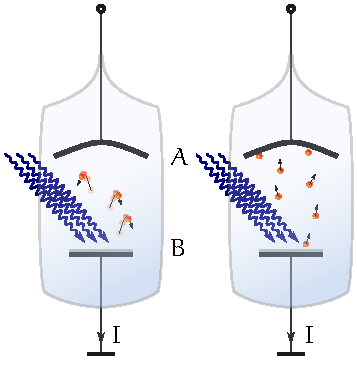
\includegraphics[width=\textwidth]{../images/The-Photoelectric-Effect/Illustration.pdf}
        \caption{\ref{source:the-photoelectric-effect} An illustration of the photoelectric effect.}
        \label{fig:the-photoelectric-effect}
    \end{figure}
    \begin{figure}[H]
        \centering
        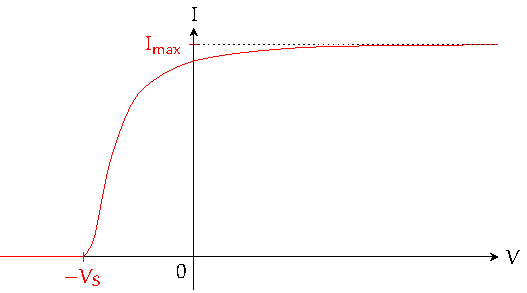
\includegraphics[width=\textwidth,page=1]{../images/The-Photoelectric-Effect/The-Photoelectric-Effect.pdf}
        \caption{\ref{source:curves-the-photoelectric-effect} An illustration of the photoelectric effect.}
        \label{fig:curves-the-photoelectric-effect}
    \end{figure}
    % \begin{figure}[H]
    %     \centering
    %     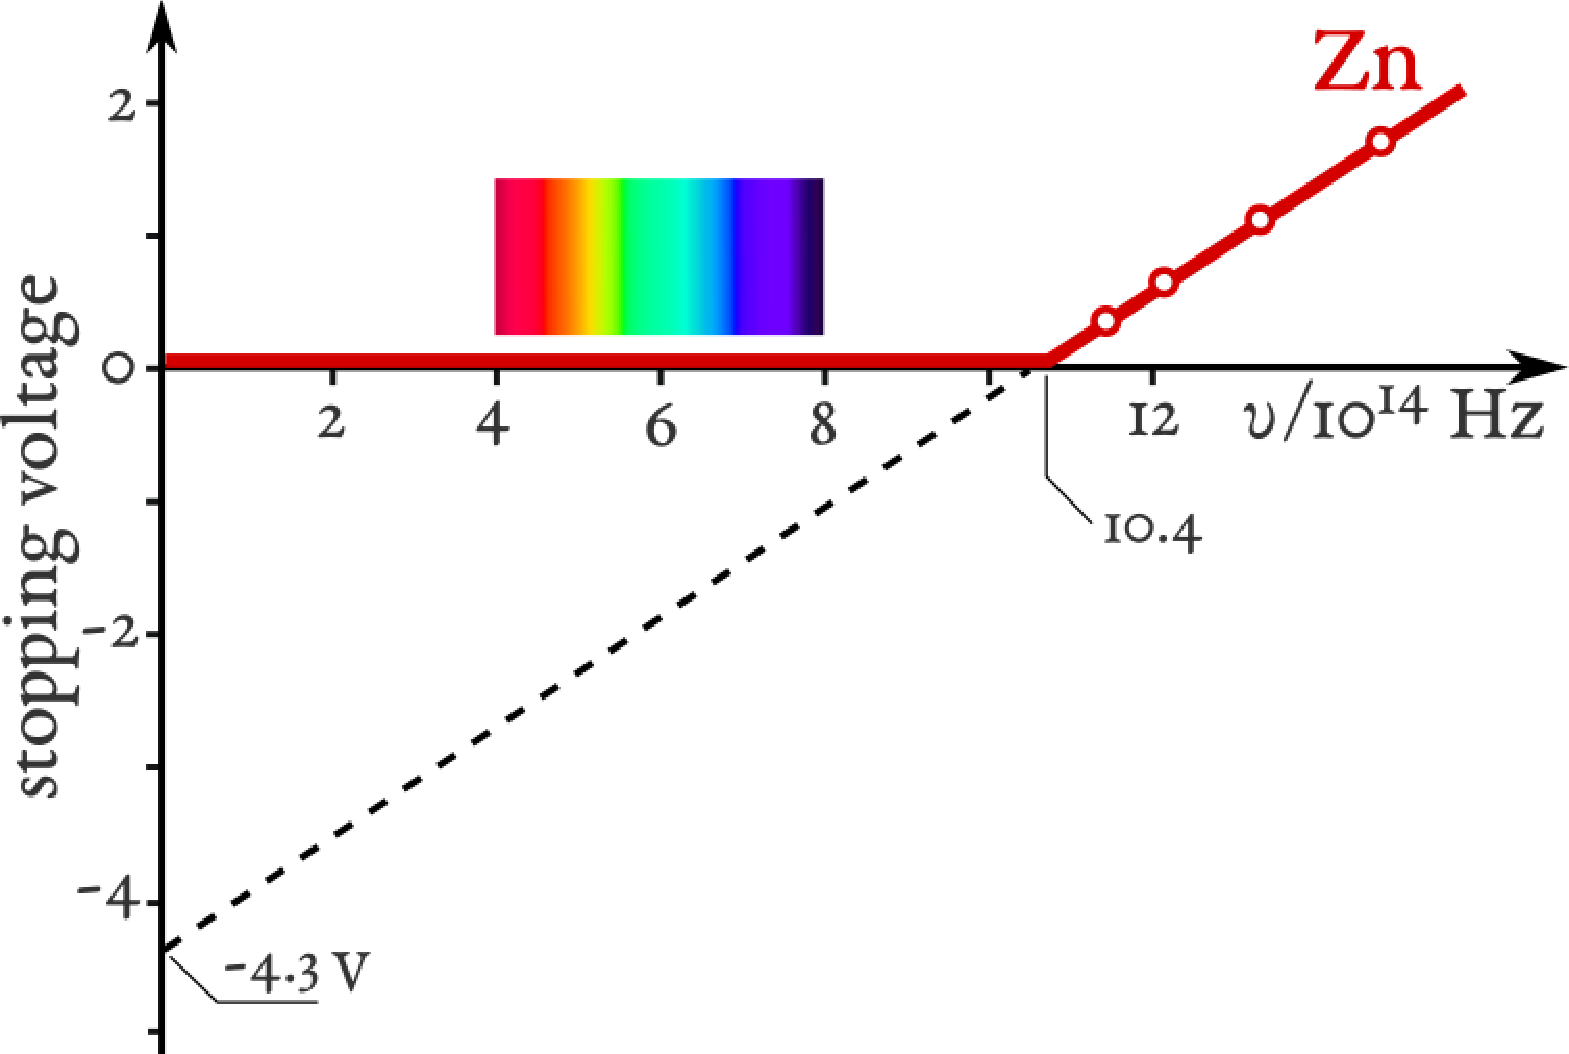
\includegraphics[width=\textwidth]{../images/Photoelectric effect stopping_voltage_diagram_for_zinc_-_English.pdf}
    %     \caption{\ref{source:max-E_k-against-frequency_zinc} The maximum kinetic energy of a photoelectron as a function of the frequency of light on zinc.}
    %     \label{fig:max-E_k-against-frequency_zinc}
    % \end{figure}
\end{minipage}%
\begin{minipage}{0.5\textwidth}
    \begin{itemize}
        \item A is negative relative to B (\(V=V_A-V_B<0\)).
        \begin{itemize}
            \item Electrons decelerate when moving towards A.
            \item If the kinetic energy \(E_k\) of an electron exceeds \(eV\), then it will reach electrode A.
            \item And when \(E_k<eV\), the electron will be repelled back to electrode A. 
            \item As \(V\) increases, more electrons have insufficient \(E_k\) to reach electrode A. i.e., less electrons reach A. So, the photocurrent is reduced.
            \item At the stopping potential \(V_s\), even the most energetic electrons have insufficient \(E_k\) to reach A. i.e. \(eV_s=E_{k,\text{max}}\). Hence, there is no photocurrent.  
        \end{itemize}
        \item A is positive relative to B (\(V=V_A-V_B>0\)).
        \begin{itemize}
            \item All electrons accelerate towards A.
            \item The saturation current is not immediately reached because some electrons' path are such that they do not hit electrode A. So, a sufficiently strong electric field is required for them to hit A.
        \end{itemize}
    \end{itemize}
\end{minipage}
% \footnotetext{Totally didn't take me 5-7 hours to tex out the next page\dots Tikz is pain, suffering, but beautiful.}
\begin{figure}[H]
    \centering
    \begin{subfigure}[c]{0.49\textwidth}
        \centering
        \includegraphics[width=\textwidth,page=2]{../images/The-Photoelectric-Effect/The-Photoelectric-Effect.pdf}
        \caption{ The maximum kinetic energy of a photoelectron plotted against the frequency of light used.}
    \end{subfigure}\hfill
    \begin{subfigure}[c]{0.49\textwidth}
        \centering
        \includegraphics[width=\textwidth,page=3]{../images/The-Photoelectric-Effect/The-Photoelectric-Effect.pdf}
        \caption{ The stopping potential for a metal surface plotted against the frequency of light used.}
    \end{subfigure}\hfill
    \begin{subfigure}[c]{0.49\textwidth}
        \centering
        \includegraphics[width=\textwidth,page=4]{../images/The-Photoelectric-Effect/The-Photoelectric-Effect.pdf}
        \caption{ The graph of photocurrent \(I\) against potential difference \(V=V_A-V_B\), under (a constant frequency but) varying intensities of light.}
    \end{subfigure}\hfill
    \begin{subfigure}[c]{0.49\textwidth}
        \centering
        \includegraphics[width=\textwidth,page=5]{../images/The-Photoelectric-Effect/The-Photoelectric-Effect.pdf}
        \caption{ The graph of photocurrent \(I\) against potential difference \(V=V_A-V_B\), under (a constant rate of photon emission but) varying frequencies of light.}
    \end{subfigure}\hfill
    \begin{subfigure}[c]{0.49\textwidth}
        \centering
        \includegraphics[width=\textwidth,page=6]{../images/The-Photoelectric-Effect/The-Photoelectric-Effect.pdf}
        \caption{The graph of photocurrent \(I\) against the intensity of light used (under a constant frequency, which exceeds the threshold).}
    \end{subfigure}\hfill
    \begin{subfigure}[c]{0.49\textwidth}
        \centering
        \includegraphics[width=\textwidth,page=7]{../images/The-Photoelectric-Effect/The-Photoelectric-Effect.pdf}
        \caption{The graph of photocurrent \(I\) against the frequency of light used (under a constant rate of photon emission).}
    \end{subfigure}\hfill
    \caption{\ref{source:curves-the-photoelectric-effect} The photoelectric effect: the relationship between the maximum kinetic energy \(E_{k,\text{max}}\), the stopping potential \(V_s\), photocurrent \(I\), potential difference \(V=V_A-V_B\), frequency \(f\) of light used, intensity of light used.}
    \label{fig:curves-TOO-the-photoelectric-effect}
\end{figure}
\begin{itemize}
    \item The \emph{de Broglie wavelength} of any particle is given by \(\lambda=h/p\).
    \item The Heisenberg Uncertainty Principle states that \(\Delta p\Delta x\gtrsim h\), where \(p\) and \(x\) are the momentum and position, respectively, of a particle. 
    \item \emph{Note.} The above applies only when considering the momentum \(p\) and position \(x\) \emph{in the same direction}. So, it is possible that, for example, \(\Delta x\Delta p_y=0\) or \(\Delta y\Delta p_x=0\).
    \item The energy of a photon involved in the transition between energy levels obeys energy conservation. i.e. \(hf=E_f-E_i\) where \(f\) is the photon's frequency.
    \item Some terminology.
    \begin{enumerate}
        \item The \emph{ground state} of an atom is the lowest state an atom can be at, such that all electrons in the atom occupy the lowest possible energy levels.
        \item An atom is said to be \emph{excited} iff one or more of its electrons are not occupying the lowest possible energy states.
        \item For this topic, \emph{ionisation} is the removal of an electron to create an ion.
        \item The \emph{ionisation energy} of an atom is the energy required for the atom to transition from the \(n=1\) to \(n=\infty\) state.
    \end{enumerate}
    \item Why do energy levels have negative values? Electrons have \emph{zero potential energy at infinity}, and so have \emph{less} potential energy (i.e. negative potential energy) near the \emph{positively} charged nucleus.
    \item[\AsteriskThin] An \emph{emission line spectrum} is a series of distinctly coloured lines against a dark background.
    \begin{figure}[H]
        \centering
        \begin{subfigure}[c]{\textwidth}
            \centering
            \pgfspectra[element=He,axis,label,label position=north west]
            \caption{The emission line spectrum of Helium.}
            \label{fig:emission-line-spectrum-helium}
        \end{subfigure}%

        \begin{subfigure}[c]{\textwidth}
            \centering
            \pgfspectra[element=H,axis,label,label position=north west]
            \caption{The emission line spectrum of Hydrogen.}
            \label{fig:emission-line-spectrum-hydrogen}
        \end{subfigure}%
        \caption{\ref{source:emission-and-absorption-lines} Some emission line spectra.}
        \label{fig:emission-lines}
    \end{figure}
    \begin{itemize}
        \item Excited atoms are unstable and de-excite by \emph{emitting} photons, eventually reaching the ground state (it does not have to immediately de-excite to the ground state).
        \item The frequency of these photons is such that \(hf=E_i-E_f\), where \(E_i\) and \(E_f\) are the initial and final energy states, respectively (\(f\) can be nonzero).
        \item Each emission spectrum is unique to each element. 
        \item Given \(n\) energy states, there will be \(\binom{n}{2}\) emission lines.
    \end{itemize}
    \item Do not use say that an atom transits from the \(n=\rule{0.5cm}{0.01mm}\) state to the \(n=\rule{0.5cm}{0.01mm}\) state, if the question does \emph{not} define \(n\).
    \item[\AsteriskThin] An \emph{absorption line spectrum} is a series of distinct dark lines against a continuous spectrum. 
    \begin{figure}[H]
        \centering
        \begin{subfigure}[c]{\textwidth}
            \centering
            \pgfspectra[element=He,axis,label,label position=north west,charge=all,absorption]
            \caption{The absorption line spectrum of Helium.}
            \label{fig:absorption-line-spectrum-helium}
        \end{subfigure}%

        \begin{subfigure}[c]{\textwidth}
            \centering
            \pgfspectra[element=H,axis,label,label position=north west,charge=all,absorption]
            \caption{The absorption line spectrum of Hydrogen.}
            \label{fig:absorption-line-spectrum-hydrogen}
        \end{subfigure}%
        \caption{\ref{source:emission-and-absorption-lines} Some absorption line spectra.}
        \label{fig:absorption-lines}
    \end{figure}
    \begin{itemize}
        \item Gaseous atoms \emph{absorb} photons with (exactly) the energies they need to transit to a higher energy state, \emph{from the ground state}. (We do not consider further excitations from above a higher energy level.)
        \item Given \(n\) energy states, there will be \(n-1\) absorption lines. 
    \end{itemize}
    \begin{example}{}{}
        State how line spectra, together with the concept of a photon, provide evidence for discrete energy levels in isolated atoms. \hspace*{\fill} [2]
        \begin{itemize}
            \item Since the emission line spectrum of an atom comprises of discrete lines, where each line corresponds to one specific wavelength \(\lambda\), the energies of photons \(E\propto 1/\lambda\) emitted are discrete. \hspace*{\fill} [1]
            \item Each photon is emitted when one electron transits from a higher energy level to a lower energy level. Since the energy level difference is equal to the energy of the emitted photon, the energy levels must be discrete. \hspace*{\fill} [1]
        \end{itemize}
    \end{example} 
    \begin{example}{}{}
        In the visible section of the spectrum of electromagnetic radiation, purple light has the shortest wavelength.
        \begin{enumerate}
            \item Calculate the energy, in eV, of a photon of purple light of wavelength \(340\cdot 10^{-9}\)m.
            \[E=hc/\lambda=\dots=3.66\mathrm{eV}.\]
            \item By reference to your answer in (i), explain why a visible line spectrum does \textbf{not} result from electrons de-exciting to the -13.6 eV energy level. \hspace*{\fill} [2]
            \begin{itemize}
                % \item The energy level difference \(E\) from the de-excitation of an electron to the -13.6 eV energy level is \emph{at least} \(13.6-\highlight[grey]{3.4}=\highlight[grey]{10.2}>3.66\mathrm{eV}\). 
                % \item An emitted photon has energy \(E\geq 3.66\mathrm{eV}>3.\)
                \item The de-excitation of an electron to the \(-13.6\) eV energy level produces a photon of minimum energy \(13.6-\rule{0.5cm}{0.01mm}=\rule{0.5cm}{0.01mm}>3.66eV={}\)energy of one purple photon. \hspace*{\fill} [1]
                \item So, an emitted photon has shorter wavelength than purple light. Since purple light has the shortest wavelength in the visible light spectrum, an emitted photon will not be in the visible light spectrum. \hspace*{\fill} [1] 
            \end{itemize}
        \end{enumerate}
    \end{example}
    \item All the light absorbed by atoms is re-emitted. Suggest why dark spectral lines are still seen: Incident light is directional, but light is re-emitted in all directions.  
    \item If an element \(_Z^AX\) lies on the \(m\)th row and in the \(n\)th group of the periodic table, then an atom of \(X\) at ground state has \(m\) electron shells and \(n\) valence electrons.
    \item The maximum number of electrons that can occupy the \(n\)th shell of an atom is \(2n^2\). 
    \begin{table}[H]
        \centering
        \begin{tabular}{ScScSc}
            \toprule
            \multicolumn{2}{Sc}{Shell} & \multirow{2}{*}[-0.7mm]{Maximum number of electrons}\\
            \cmidrule{1-2}
            Number & Letter &\\
            \midrule
            1st & \(K\) & 2\\
            2nd & \(L\) & 8\\
            3rd & \(M\) & 18\\
            4th & \(N\) & 32\\
            \bottomrule
        \end{tabular}
        \caption{The maximum number of electrons that can occupy the first four shells of an atom.}
        \label{table:maximum-number-of-electrons-in-shell}
    \end{table}
    % ^ Source: https://education.jlab.org/qa/electron_number.html 
    % \item Similarity: The distinct lines in both spectra, for the same atoms, are of the \emph{same wavelengths}.
    \item Similarity: All distinct lines in an absorption line spectrum are present and of the \emph{same wavelengths} in an emission line spectrum for the same atoms.
    \item Difference: There are at least as many emission lines as there are absorption lines. In general, there are \emph{more} emission lines. 
    \item \emph{Note.} It is critical to accurately represent the distance between the each emission line (or absorption line), especially the one furthest away from adjacent lines. E.g. the line near the 660 nm mark in Figure \ref{fig:emission-line-spectrum-hydrogen} or \ref{fig:absorption-line-spectrum-hydrogen}. 
\end{itemize}
\begin{figure}[H]
    \centering
    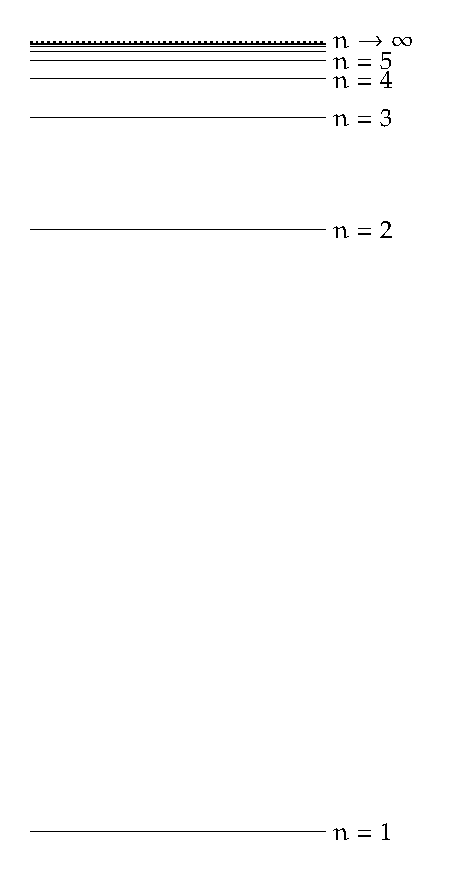
\includegraphics[height=0.5\textheight,angle=90]{../images/Energy-Level/Energy-Level.pdf}
    \caption{\ref{source:hydrogen-energy-levels} The energy levels of Hydrogen (drawn to scale).}
    \label{fig:hydrogen-energy-levels}
\end{figure}
\newpage
\null
\vfill
\begin{figure}[H]
    \centering
    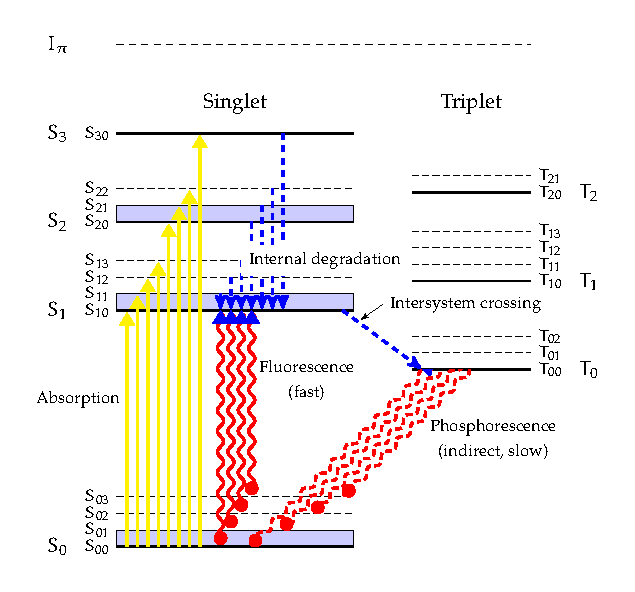
\includegraphics[width=\textwidth,page=1]{../images/Energy level diagram(s)/energy-level-1.pdf}
    \caption{\ref{source:fluor-energy-levels} (Pretty diagram; \emph{out of syllabus}) Typical energy levels for $\pi$-orbitals of a fluor molecule. Spin singlet~($S$) and triplet~($T$) states are separated for clarity. The ionization level $I_\pi$ is shown at the top.  Excited states as well as vibrational sublevels (dashed horizontal lines) are shown. Internal degradation is a non-radiative process, while fluorescence and phosphorescence are radiative decays.  The decay $T_0 \to S_0$, however, is indirect, by interactions with other molecules.}
    \label{fig:fluor-energy-levels}
\end{figure}
\vfill
\newpage
\null
\vfill
\begin{figure}[H]
    \centering
    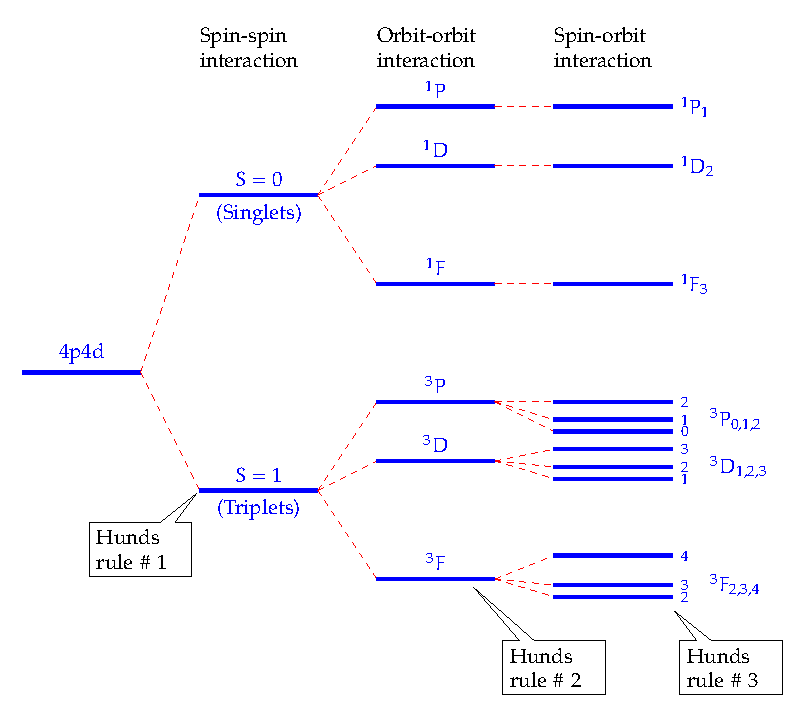
\includegraphics[width=\textwidth]{../images/Energy level diagram(s)/energy-level-3.pdf}
    \caption{\ref{source:hunds} (Another pretty diagram; \emph{out of syllabus}) An illustration of Hund's rule.}
    \label{fig:hunds}
\end{figure} 
\vfill
\newpage
\begin{minipage}{0.6\textwidth}
    \begin{figure}[H]
        \centering
        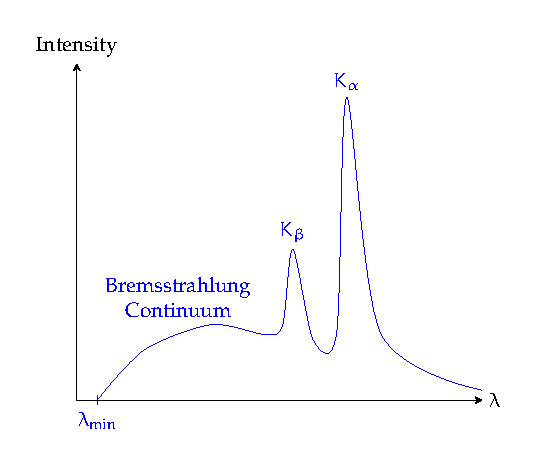
\includegraphics[width=\textwidth]{../images/x-ray-spectrum/x-ray-spectrum.pdf}
        \caption{\ref{source:x-ray-spectrum} \(X\)-ray spectrum.}
        \label{fig:x-ray-spectrum}
    \end{figure}
\end{minipage}%
\begin{minipage}{0.4\textwidth}
    \begin{figure}[H]
        \centering
        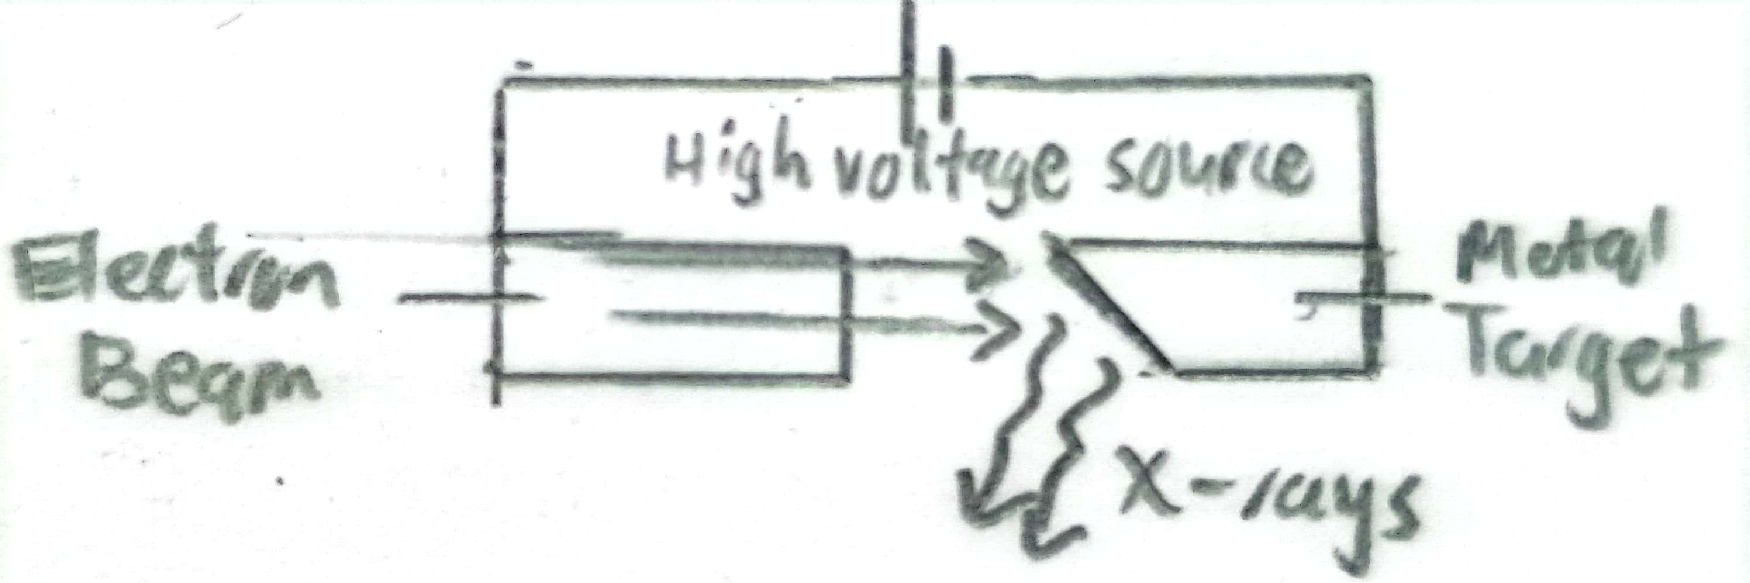
\includegraphics[width=\textwidth,angle=90]{../images/x-ray-apparatus.pdf}
        \caption{\ref{source:x-ray-apparatus} Experimental set-up to produce \(X\)-rays}
        \label{fig:x-ray-apparatus}
    \end{figure} 
\end{minipage}
\begin{longtable}{m{0.25\textwidth}m{0.75\textwidth}}
    \toprule
    \begin{minipage}{0.25\textwidth}
        \centering
        Features
    \end{minipage}& 
    \begin{minipage}{0.75\textwidth}
        \centering
        Explanation
    \end{minipage}\\
    \midrule
    A sharp cut-off / minimum wavelength \(\lambda_{\text{min}}\)& 
    % When the kinetic energy of an incident electron is fully lost as a single photon, that photon has maximum kinetic energy.
    \begin{itemize}
        % \item An X-ray photon has maximum kinetic energy --- i.e. has minimum wavelength \(\lambda_{\text{min}}\) --- when the kinetic energy of an incident electron is fully lost as that photon. i.e. \(E_k=hc/\lambda_{\text{min}}\).
        % \item Furthermore, each incident electron has kinetic energy \(E_k=eV\).
        % \item So, we solve \(hc/\lambda_{\text{min}}=eV\), telling us that \(\lambda_{\text{min}}=\frac{hc}{eV}\).
        % \item No emitted X-ray photon has a lower wavelength \(\lambda<\lambda_{\text{min}}\), because such a photon would have 
        % energy exceeding \(hc/\lambda_{\text{min}}\), and hence, exceeding the kinetic energy of all incident electrons. 
        % % energy \(hc/\lambda>hc/\lambda_{\text{min}}=E_k=eV\), and hence, require a more energetic electron --- i.e. an electron accelerated through a larger potential difference \(V\)
        \item Incident electrons are accelerated through an electric potential \(V\), giving them a maximum kinetic energy of \(E_k=eV\). 
        \item When such an electron is decelerated and loses all its \(E_k\), it emits a single X-ray photon of maximum possible energy, corresponding to the minimum wavelength seen on the spectrum. 
        \item By the conservation of energy, \(eV=\frac{hc}{\lambda_{\text{min}}}\) so \(\lambda_{\text{min}}=\frac{hc}{eV}\).
    \end{itemize}\\
    \midrule
    A broad continuous spectrum known as the \emph{Bremsstrahlung continuum}. (Bremsstrahlung is braking radiation in German.)&
    \begin{itemize}
        \item When high speed incident electrons pass by the (positively) charged nuclei of the high atomic mass lead atoms, the strong (attractive) electric forces lead to a sudden, large deceleration of the electrons.
        \item Their kinetic energies are lost through the emission of Bremsstrahlung X-ray photons.
        % , which are \(X\)-ray photons of a range of energies.
        \item Since the magnitude of the deceleration, and hence the magnitude of change in kinetic energy, experienced by the incident electrons varies continuously and is not discrete, the wavelengths of the emitted photons have a continuous distribution.
        \item Hence, Bremsstrahlung produces a continuous spectrum of electromagnetic radiation. 
    \end{itemize}\\
    \midrule
    \newpage
    \midrule
    Sharp peaks \(K_\alpha\) and \(K_\beta\) called characteristic lines/X-rays. &
    \begin{itemize}
        \item An accelerated incident electron `collides' with an electron from the innermost \(K\)-shell, kicking it out of the shell.
        \item The atom is excited due to the vacancy in the \(K\)-shell.
        \item An electron from the higher energy shell transits to the \(K\)-shell, emitting a photon.
        \item
        \begin{tabular}{ScScScScSc}
            \toprule
            Series & Line & Initial shell \((m)\) & Final shell \((n)\) & \(m-n\)\\
            \midrule
            \multirow{2}{*}{\(K\) series} & \(K_\alpha\) & \(L\)-shell (2nd) & \multirow{2}{*}{\(K\)-shell (1st)} & 1\\
            & \(K_\beta\) & \(M\)-shell (3rd) && 2\\
            \midrule
            \multirow{2}{*}{\(L\) series} & \(L_\alpha\) & \(M\)-shell (3rd) & \multirow{2}{*}{\(L\)-shell (2nd)} & 1\\
            & \(L_\beta\) & \(N\)-shell (4th) && 2\\
            \bottomrule
        \end{tabular}
            \item See Figure \ref{fig:X-ray-series} for an illustration. 
            \item Every element has a unique set of energy levels, and hence, characteristic lines.
        \end{itemize}\\
    \bottomrule
    \caption{The features of an X-ray spectrum.}
\end{longtable}
\begin{figure}[H]
    \centering
    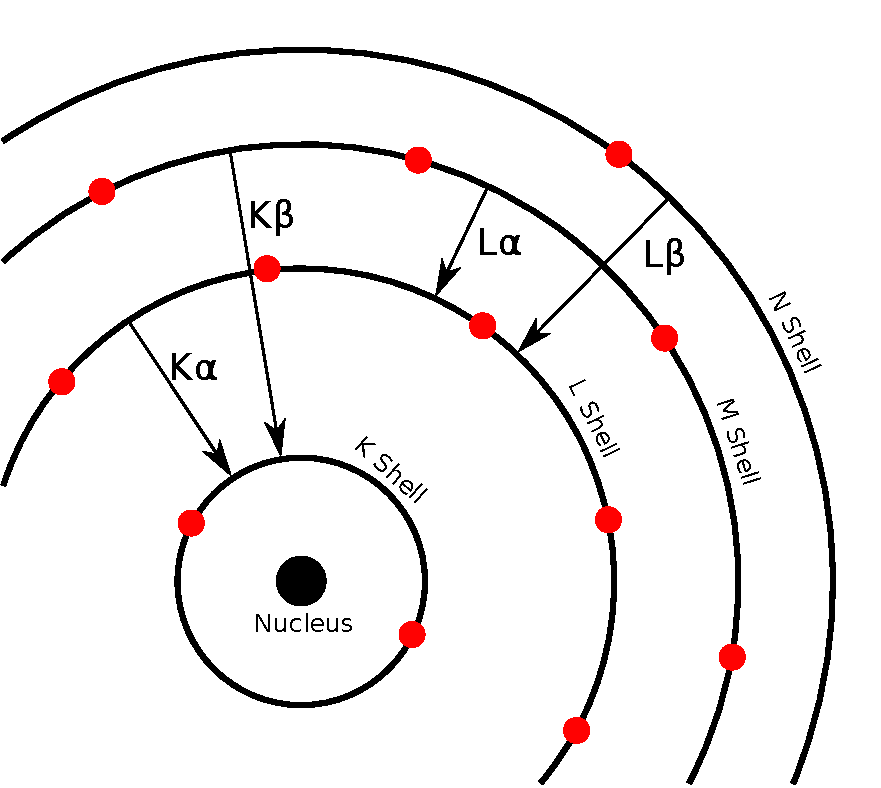
\includegraphics[width=0.75\textwidth]{../images/CharacteristicRadiation.pdf}
        \caption{\ref{source:X-ray-series} X-ray series}
        \label{fig:X-ray-series}
\end{figure}